\section{Equazioni differenziali}
\subsection{Definizioni}
Un'equazione differenziale è una relazione tra una funzione incognita $y=y(t)$ e alcune sue derivate.\newline
\newline
Si dice \textbf{equazione differenziale di ordine} $n$ un equazione del tipo:
\[
    F(t, y(t), y'(t), y''(t), \dots, y^{(n)}(t)) = 0 \;\;\;\;\;\;\;(t \in I)
\]
dove $y(t)$ è la funzione incognita.\newline
\newline
Si dirà \textbf{soluzione}, o (curva) integrale, di un equazione differenziale, nell'intervallo $I$, una funzione $\phi(t)$, definita almeno in $I$ (ma in generale può essere definita in $J \subseteq I$) e a valori reali per cui risulti
\[
    F(t, \phi(t), \phi'(t), \phi''(t), \dots, \phi^{(n)}(t))= 0 \;\;\;\;\;\;\;\; \;\forall\;t \in J
\]
\ \newline
\newline
Diremo che un'equazione differenziale è in \textbf{forma normale} se è possibile esplicitare la derivata di ordine massimo in funzione di tutte le derivate di ordine inferiore:
\[
    y^{(n)}(t) = g(t,y(t),y'(t),y''(t), \dots, y^{(n-1)}(t)) \;\;\;\;\;\;\;(t \in I)
\]
\ \newline
\newline
\textbf{Problema di Cauchy}:
Data un'equazione in forma normale
\[
    y^{(n)}(t) = g(t,y(t),y'(t),y''(t), \dots, y^{(n-1)}(t)) \;\;\;\;\;\;\;(t \in I)
\]
a essa vengono associate $n$ delle condizioni
\[
    y(t_0) = y_0 \;\;\;\;\; y'(t_0)=y_1 \;\;\;\;\;\dots \;\;\;\;\;y^{(n-1)}(t_0) = y_{n-1}
\]
dove $t_0$ rappresenta l'istante iniziale e $y_0,\dots,y_{n-1}$ rappresentano lo stato. Risolvere un problema di Cauchy significa riuscire a prevedere come si comproterà la $y(t)$ (stato del sistema) negli istanti futuri $t>t_0$. Per risolvere un problema di Cauchy si intende sempre che bisogna trovare come soluzione una funzione:
\begin{itemize}
    \item definita su un intervallo $I$, contenente il punto $t_0$;
    \item derivabile in tutto $I$ e che soddisfa l'equazione in tutto $I$.
\end{itemize}
\ \newline
Chiameremo \textbf{integrale generale} di un'equazione differenziale l'insieme di tutte le sue infinite soluzioni; chiameremo invece \textbf{integrale particolare} una sua soluzione che soddisfa particolari proprietà quali, ad esempio, quelle imposte dal problema di Cauchy.\newline
\newline
L'integrale generale è ricavabile dall'equazione in forma normale con vari metodi che vediamo più avanti, mentre le varie condizioni permettono di ricavare un integrale particolare.
\subsection{Esistenza e unicità}
In questo paragrafo studiamo l'esistena e l'unicità per il problema di Cauchy nel caso di equazioni differenziali del prim'oridne in forma normale. Se un equazione fosse di ordine superiore, ad esempio del second'ordine $y'' = f(t,y,y')$, con un semplice trucco potremmo ricondurci a un sistema del prim'ordine: basta porre $z = y'$ e la precedente equazione del second'ordine si traduce nelle due seguenti equazioni del prim'ordine: $y'=z$ e $z' = f(t,y,z)$,  dove l'incognita è adesso il vettore $(y,z)$.\newline
\newline
\textbf{teor.} \textbf{Teorema di Peano}:\newline
Sia $\Omega \subset \mathbb{R}^2$ un aperto e sia $(t_0, y_0) \in \Omega$. Se $f \in C^0 (\Omega)$ allora esiste una soluzione del problema di Cauchy:
\[
    \begin{cases}
        y' = f(t,y)\\ y(t_0) = y_0
    \end{cases}
\]
\ \newline
\textbf{teor.} \textbf{Teorema di Cauchy}:\newline
Sia $\Omega \subset \mathbb{R}^2$ un aperto e sia $(t_0, y_0) \in \Omega$. Se $f,f_y \in C^0(\Omega)$, allora esiste un'unica soluzione del problema di Cauchy:
\[
    \begin{cases}
        y' = f(t,y)\\ y(t_0) = y_0
    \end{cases}
\]
\subsection{Equazioni del primo ordine}
Analiziamo ora vari metodi per risolvere il problema di Cauchy per equazioni del prim'ordine:
\[
    \begin{cases}
        y' = f(t,y)\\ y(t_0) = y_0
    \end{cases}
\]
\subsubsection{Equazioni a variabili separabili}
Un'equazione differenziale del tipo
\[
    y' = f(t)g(y)
\]
si dice \textbf{equazione a variabili separabili}.\newline
\newline
Dai teoremi di Cauchy e di Peano ricaviamo il seguente \textbf{corollario}:\newline
Siamo $t_0,y_0 \in \mathbb{R}$ e sia $f$ continua in un intorno di $t_0$:
\begin{itemize}
    \item Se $g$ è continua in un intorno di $y_0$, allora il problema di Cauchy $y(t_0) = y_0$ per l'equazione a variabili separabili $y'=f(t)g(y)$ ammette una soluzione.
    \item Se $g$ è di classe $C^1$ in un intorno di $y_0$, allora il problema di Cauchy $y(t_0) = y_0$ per l'equazione a variabil iseparabili $y'=f(t) g(y)$ ammette una e una sola soluzione.
\end{itemize}
\ \newline
Come prima cosa, osserviamo che se esiste $\bar{y} \in \mathbb{R}$ tale che $g(\bar{y}) = 0$ allora $y(t) \equiv \bar{y}$ è una soluzione costante dell'equazione a variabili separabili; pertanto, se all'equazione a variabili separabili associamo il problema di cauchy $y(t_0) = \bar{y}$ abbiamo già trovato una soluzione (naturalmente se $g$ è solo continua potrebbero essercene altre). Ma supponiamo di considerare un problema di cauchy $y(t_0) = y_0$ con $g(y_0) \neq 0$, in modo da poter dividere l'intera equazione a variabili separabili per $g(y)$ (almeno in un intorno di $y_0$). Usando la notazione $y' = \frac{dy}{dt}$, i semplici passaggi per risolvere l'equazione a variabil iseparabili $y' = f(t) g(y)$ sono i seguenti:
\[
    \frac{dy}{dt} = f(t) g(y) \Longrightarrow \frac{dy}{g(y)} = f(t) dt \Longrightarrow \int \frac{1}{g(y)}dy = \int f(t) dt
\]
A questo punto, una volta risolti gli integrali, è sufficiente esprimere $y$ in funzione di tutto il resto: quindi se $G(y)$ è una primitiva di $\frac{1}{g(y)}$ e $F(t)$ è una primitiva di $f(t)$, otteniamo
\[
    G(y) = F(t) + c
\]
e se si può ottenere la funzione inversa di $G$ possiamo scrivere;
\[
    y = G^{-1}(F(t) + c)
\]
Notiamo che gli integrali fanno comparire una costante arbitraria che verrà determinata tramite le condizioni importe dal problema di Cauchy.
\newline
\newline
\textbf{Procedimento per risolvere equazioni a variabili separabili}:
\begin{itemize}
    \item stabilire se $f,g \in C^0$ o se $g \in C^1$;
    \item risolvere l'equazione $g(\bar{y}) = 0$;
    \item tutte le soluzioni di questa equazione rappresentano soluzioni costanti;
    \item se $g \notin C^1$ ci potrebbe essere un pennello di Peano che si stacca dalla soluzione costante;
    \item se $g \in C^1$ c'è unicità e le soluzioni costanti rappresentano dei "limiti invalicabili" per le altre soluzioni;
    \item risolvere il problema di Cauchy.
\end{itemize}
\subsubsection{Note sugli esercizi: Insieme di definizione di un problema ci Cauchy per equazioni a variabili separabili}
Dato un problema di Cauchy per un'equazione a variabili separabili
\[
    \begin{cases}
        y' = f(t) g(y) \\ y(t_0) = y_0
    \end{cases}
\]
la teoria garantisce che se $a(t)$ è continua in un intorno di $t = t_0$ e le funzioni $b(y), b'(y)$ sono continue in un intorno di $y_0$ allora esiste un'unica soluzione al problema di Cauchy, definita in un intorno di $t_0$ (contenuto nell'intorno di $t_0$ relativo alla funzione $a(t)$).
\subsubsection{Equazioni lineari (derivata di un prodotto; sovrapposizione e variazione delle costanti arbitrarie)}
Un'equazione differenziale del tipo
\[
    y' = a(t) y + b(t)
\]
si dice \textbf{equazione lineare}.\newline
\newline
Dal teorema di Cauchy ricaviamo il seguente \textbf{corollario}:\newline
Siano $t_0,y_0 \in \mathbb{R}$ e siano $a,b$ continue in un intorno di $t_0$. Allora il problema di Cauchy $y(t_0) = y_0$ per l'equazione differenziale lineare ammette una e una sola soluzione.\newline
\newline
Per trovare l'integrale generale ci sono due metodi:
\begin{itemize}
    \item \textbf{Primo metodo: derivata di un prodotto}:\newline
    Data $y' = a(t) y + b(t)$, sia $A(t) = \int a(\tau)d \tau$ una qualunque primitiva di $a(t)$. Trasportando a primo membro il termine $a(t) y$ e moltiplicando per l'esponenziale $e^{-A(t)}$, possiamo riscrivere l'equazione differenziale lineare nella forma:
    \[
        e^{-A(t)} y'(t) - e^{-A(t)}a(t) y(t) = e^{-A(t)}b(t).
    \]
    In questa forma, a primo membro riconosciamo la derivata di un prodotto:
    \[
        \frac{d}{dt} \left( e^{-A(t)} y(t) \right) = e^{-A(t)} b(t).
    \]
    Integrando ambo i membri si ottiene
    \[
        e^{-A(t)} y(t) = \int e^{-A(\tau)} b(\tau) d \tau + C
    \]
    dove con $C \in \mathbb{R}$ abbiamo indicato la generica costante dovuta all'integrale indefinito. Moltiplicando per l'esponenziale otteniamo infine
    \[
        y(t) = e^{A(t)}\left\{ \int e^{-A(\tau)} b(\tau) d \tau + C \right\}.
    \]
    La soluzione di un problema di Cauchy si ottiene imponendo la condizione iniziale $y(t_0) = y_0$.
    \textbf{oss.} Non imparare a memoria la formula ! E' facile confondersi con i segni di $A$.
    \item \textbf{Secondo metodo: sovrapposizione e variazione delle costanti arbitrarie}:\newline
    Data $y' = a(t) y + b(t)$, per prima cosa risolviamo l'\textbf{equazione omogenea} associata, che si ottiene ponendo $b(t) = 0$ e che quindi è $y' = a(t) y$. Ovviamente $t \equiv 0$ è soluzione. Per $y\neq 0$, diventa un equazione a variabili separabili che, stando a quanto visto precedentemente si risolve come
    \[
        \frac{dy}{dt} = a(t) y \Rightarrow \frac{dy}{y} = a(t) dt \Rightarrow  log|y| = A(t) + c \Rightarrow |y(t)| = Ce^{A(t)}
    \]
    dove $c \in \mathbb{R}$ e $A$ è una primitiva di $a$.\newline
    \newline
    Possiamo quindi affermare che tutte le soluzioni dell'equazione $y'=a(t) y$ sono $y(t) = Ce^{A(t)}$ con $C \in \mathbb{R}$.\newline
    \newline
    Vale il \textbf{principio di sovrapposizione}:\newline
    L'integrale generale dell'equazione $y' = a(t) y + b(t)$ si ottiene sommando all'integrale generale dell'equazione omogenea associata un integrale particolare di $y' = a(t) y + b(t)$.\newline
    \newline
    Resta dunque da determinare una soluzione dell'equazione completa $y' = a(t) y + b(t)$. Per trovarla sfruttiamo il \textbf{metodo della variazione delle costanti arbitrarie}. La costante che faremo variare è $C$ che compare in $Ce^{A(t)}$: supponiamo cioè che anzichè essere una costante sia una funzione e cerchiamo l'integrale particolare di $y' = a(t) y + b(t)$ nella forma $y_1(t) = C(t) e^{A(t)}$. Imponendo a questa funzione di soddisfare $y' = a(t) y + b(t)$ si trova
    \begin{align*}
        y'_1= a(t)y_1 + b(t) \Rightarrow C'(t) e^{A(t)} + C(t)a(t)e^{A(t)} = C(t) a(t) e^{A(t)} + b(t) \Rightarrow \\
        \Rightarrow C'(t) e^{A(t)} = b(t) \Rightarrow C'(t) = b(t) e^{-A(t)} \Rightarrow C(t) = \int b(\tau) e^{-A(\tau)} d \tau
    \end{align*}
    Abbiamo così trovato l'integrale particolare $y_1(t) = e^{A(t)} \int b(\tau) e^{-A(\tau)} d \tau$ che, sommato all'integrale generale dell'equazione omogenea $Ce^{A(t)}$, fornisce lo stesso risultato che abbiamo ottenuto col primo metodo della derivata di un prodotto:
    \[
        y(t) = e^{A(t)}\left\{ \int e^{-A(\tau)} b(\tau) d \tau + C \right\}.
    \]
\end{itemize}
\ \newline
\textbf{Riassunto: equazioni lineari in breve}\newline
\textbf{teor.} Problema di Cauchy per un equazione lineare del prim'ordine.\newline
Siano $a, f$ funzioni continue in un intervallo $I$ contenente $t_0$. Allora, per ogni $y_0 \in \mathbb{R}$ il problema di Cauchy
\[
    \begin{cases}
        y'(t) + a(t)y(t)= f(t)\\
        y(t_0) = y_0
    \end{cases}
\]
ha una e una sola soluzione $y \in C^1(I)$ e tale soluzione è
\[
    y(t) = ce^{-A(t)} + e^{-A(t)} \int_{t_0}^{t} f(s)e^{A(s)}ds
\]
\subsubsection{Note sugli esercizi: Insieme di definizione di un problema ci Cauchy per equazioni lineari del prim'ordine}
Dato il problema di Cauchy
\[
    \begin{cases}
        y'= a(t) y + b(t)\\ y(t_0) = y_0
    \end{cases}
\]
la teoria garantisce che, se le funzioni $a(t)$ e $b(t)$ sono continue in un intervallo $I$ aperto contenente $t_0$, allora esiste una e una sola soluzione dell'equazione differenziale data che soddisfi anche la condizione $y(t_0) = y_0$, tale soluzione sarà definita per $t \in I$.\newline
Una volta calcolata $y(t)$ (cioè dopo aver trovato l'integrale generale $y(t)$ e averci sostituito il valore di $C$ trovato tramite la condizione $y(t_0) = y_0$) essa è soluzione di un problema di Cauchy nell'intervallo aperto più grande contenente $t_0$ e in cui è definita continua e derivabile.
\newline
\newline
Analiziamo l'approccio da seguire:\newline
\newline
Per trovare l'\textbf{insieme di definizione della soluzione del problema di Cauchy} innanzitutto si controlla dove è definita e continua l'equazione di partenza $y' = a(t) y + b(t)$:
\begin{itemize}
    \item Se $t_0$ non appartiene all'insieme appena trovato, allora la teoria non permette di dire nulla circa l'esistenza di una soluzione.
    \item Se $t_0$ appartiene all'insieme appena trovato la teoria ci dice che la soluzione esiste.
\end{itemize}
In ogni caso si procede col calcolo dell'integrale generale $y(t)$ e a trovare la soluzione del problema di Cauchy (si cerca il valore della costante $C$, imponendo il passaggio dell'integrale generale $y(t)$ per il punto definito dalla condizione di Cauchy $y(t_0) = y_0$).
\newline
\newline
A questo punto per determinare l'insieme di definizione in cui questa soluzione sia valida bisogna prendere l'\textbf{intervallo} (cioè un insieme continuo) contenente il punto $t_0$ per cui la soluzione $y(t)$ e l'equazione di partenza $y'= a(t)y + b(t)$ (che rappresenta la derivata della soluzione) siano continue e definite.
\newline
\newline
La ricerca dell'intervallo di definizione non finisce qui: c'è la possibilità di \textbf{prolungare per continuità} la soluzione in un intervallo più grande. Invece di stabilire l'intervallo in cui la soluzione sia valida nei domini di $y(t)$ e $y' = a(t) y + b(t)$, lo cerchiamo \textbf{dove la soluzione $y(t)$ è continua e derivabile} (in alcuni casi la derivata della soluzione ha un insieme di definizione "più grande" di quello dell'equazione differenziale di partenza $y' = a(t)y + b(t)$, questo effetto è dovuto al fatto che la costante $C$. che sostituiamo nella soluzione, modifica la soluzione e in alcuni casi "fa sparire" i termini fastidiosi che limitano il dominio).
\subsubsection{Equazioni omogenee}
Un'equazione differenziabile si dice \textbf{omogenea} se si può scrivere nella forma
\[
    y'=f(\frac{y}{t}).
\]
\ \newline
Dal teorema di Cauchy ricaviamo il seguetne \textbf{corollario}:\newline
Siano $t_0, y_0 \in \mathbb{R}$ e sia $f \in C^1$ in un intorno di $\frac{y_0}{t_0}$. Allora il problema di Cauchy $y(t_0) = y_0$ per l'equazione omogenea ammette una e una sola soluzione.\newline
\newline
La fomra stessa di un equazione omogenea richiede una certa prudenza nello scegliere $t_0 = 0$ come istante iniziale. In realtà la stessa prudenza va usata anche per $y_0 = 0$, dato che, ad esempio, anche l'equazione $y'=\frac{t}{y}$ è omogenea.\newline
\newline
Per trovare l'integrale generale dell'equazione omogenea, la si riconduce a un'equazione a variabili separabili. Si pone
\[
    z(t) = \frac{y(t)}{t} \Rightarrow y(t) = t z(t) \Rightarrow y'8t) = z(t) + tz'(t)
\]
e l'equazione omogenea diventa
\[
    z + tz' = f(z) \Rightarrow  z' = \frac{f(z) -z}{t} \Rightarrow  \frac{dz}{f(z) - z} = \frac{dt}{t}
    \Rightarrow  \int \frac{dz}{f(z) -z} = log|t| + c.
\]
A questo punto, è enecessario risolvere l'equazione $f(z) = z$; se esiste $k \in \mathbb{R}$ tale che $f(k) = k$, allora $z(t) \equiv k$ è soluzione e, diconseguenza, $y(t) = kt$ è soluzione dell'equazione omogenea. Se $f \in C^1$, la retta che rappresenta tale funzione diventa un limite invalicabile per le altre soluzioni. Esclusi questi valori di $k$, l'equazione è diventata a variabili separabili.
\subsubsection{Equazione di Bernoulli}
Un equazione differenziale si dice di \textbf{Bernoulli} se si può scrivere nella forma
\[
    y' = a(t)y + b(t) y^\alpha \;\;\;\;\;\;\;(\alpha \in \mathbb{R})
\]
osserviamo subito che se $\alpha=0$ o $\alpha = 1$ l'equazione è lineare (e possiamo risolverla con il metodo della derivata di un prodotto o il metodo di sovrapposizione e variazione delle costanti arbitrarie). Se poi $\alpha$ fosse irrazionale o razionale con denominatore pari, non avrebbe senso definire $y^\alpha$ per $y < 0$. Infine, se $\alpha < 0$ non ha senso $y^\alpha$ per $y=0$.\newline
\newline
Per evitare complicazioni ci occuperemo solo di soluzioni non negativa ($y \geq 0$).\newline
\newline
Dal teorema di cauchy ricaviamo il seguente \textbf{corollario}:\newline
Siano $t_0 \in \mathbb{R}$, $y_0 \geq 0$ e siano $a,b \in C^0$ in un intorno di $t_0$. Allora il problema di Cauchy $y(t_0) = y_0$ per un equazione di Bernoulli ammette una e una sola soluzione nei seguenti casi:
\begin{itemize}
    \item $\alpha> 1 \;\;\;\;\; y_0 \geq 0$
    \item $0< \alpha< 1 \;\;\;\;\;y_0 > 0$
    \item $\alpha<0 \;\;\;\;\;y_0 > 0$
\end{itemize}
Se $\alpha > 0$ l'equazione di bernoulli ammette anche la soluzione nulla $y \equiv 0$, pertanto se  $\alpha > 1$ e $y_0 = 0$, il problema di Cauchy ammette solo la soluzione nulla.\newline
Nel caso $y_0 = 0$ e $0<\alpha < 1$, è garantita l'esistenza di una soluzione per il problema di Cauchy $y(t_0) = 0$ ma non ne è assicurata l'unicità (potrebbe crearsi un pennello di Peano).\newline
Se $y_0 > 0$ la soluzione rimarrà strettamente positiva per $\alpha > 1$, potrenne agganciarsi alla soluzione $y= 0$ con un pannello di peano se $0< \alpha<1$, potrebbe tendere a $0$ con tangente verticale se $\alpha<0$ (in quest'ultimo caso, bisogna verificare il comportamento della funzione $b(t)$ che, annullandosi, potrebbe verificare l'infinito di $y^\alpha$).\newline
\newline
\textbf{Risolvere un equazione di Bernoulli}:\newline
Si divide l'equazione per $y^\alpha$ e si ottiene $y^{-\alpha} y' = a(t) y^{1-\alpha} + b(t)$.\newline
Si pone $z(t) = y(t)^{1-\alpha}$ e si ottiene $z' = (1-\alpha)a(t)z + (1-\alpha) b(t)$, che è un'equazione lineare e quindi possiamo risolvere con i soliti metodi. Una volta trovata la soluzione $z(t)$ (che sarà $\geq 0$ o $>0$ a seconda dei valori di $\alpha$), si determina $y(t) = z(t)^{\frac{1}{1-\alpha}}$.
\subsubsection{Prolungamento delle soluzioni}
Sia $f, f_y \in C^0\left( (a,b) \text{x} \mathbb{R} \right)$ e supponiamo che esistano due costanti $k_1,k_2 > 0$ tali che 
\[
    |f(t,y)| \leq k_1 + k_2 |y| \;\;\;\;\; \;\forall(t,y) \in(a,b)\text{x}\mathbb{R}
\]
Allora per ogni $(t_0,y_0) \in(a,b) \text{x} \mathbb{R}$ lìunica soluzione del problema di Cauchy di prim'ordine è prolungabile a tutto l'intervallo $(a,b)$.
\subsection{Equazioni lineari del secondo ordine a coefficienti costanti}
\subsubsection{Integrale generalea dell’equazione omogenea e integrale
particolare dell’equazione completa}
Consideriamo l'equazione differenziale 
\[
    ay''(t) + by'(t) + cy(t) = f(t) \;\;\;\;\;\;\;t \in I
\]
dove $a,b,c \in \mathbb{R}$ e $f \in C^0(I)$. Se fosse $a=0$, questa equazione sarebbe del prim'ordine. Se $a\neq0$ possiamo dividere per $a$ e ottenere un'equazione del tipo
\[
    y''(t) + by'(t) + cy(t) = f(t) \;\;\;\;\;\;\; t \in I.
\]
Questa è un'\textbf{equazione lineare del second'ordine a coefficienti costanti}.\newline
\newline
Analogamente a quanto visto per il metodo di sovrapposizione e variazione delle costanti per le equazioni lineari di prim'ordine, vale il principio di sovrapposizione:\
L'\textbf{integrale generale} di $y''(t) + by'(t) + cy(t) = f(t)$ si ottiene sommando all'integrale \textbf{generalea} dell'equazione \textbf{omogenea} un integrale \textbf{particolare} dell'equazione \textbf{completa}:
\begin{itemize}
    \item Vediamo dunque come risolvere l'\textbf{equazione omogenea associata}:
    \[
        y'' + by' + cy = 0 \;\;\;\;\;\;\;t \in I
    \]
    Dato che quest'equazione si può ricondurre a un sistema di due equazioni del prim'ordine, il problema di cauchy da associare sarà del tipo
    \[
        y(t_0) = y_0, \;\;\;\;\;\;\;y'(t_0)=y_1.
    \]
    Questo significa che, oltre alal posizionei niziale $y(t_0)$, è necessario imporre una variazione iniziale $y'(t_0)$, in questo modo il teorema di Cauchy nella versione per i sistemi, garantisce che ci sia un'unica soluzione.\newline
    Le due condizioni imposte mostrano che le soluzioni hanno \textbf{due gradi di libertà}: l'integrale generale è uno spazio vettoriale di dimensione $2$. basta quindi trovare due soluzioni non proporzionali.\newline
    Iniziamo sostituendo $y(t) = e^{\lambda t}$ e otteniamo
    \[
        e^{\lambda t} (\lambda^2 + b \lambda + c) = 0.
    \]
    L'equazione 
    \[
        \lambda^2 + b \lambda + c = 0
    \]
    viene chiamata \textbf{equazione caratteristica} associata e si possono verificare tre casi:
    \begin{itemize}
        \item $b^2 > 4c$: in tal caso, l'equazione caratteristica ammette due soluzioni reali $\lambda_1, \lambda_2 \in \mathbb{R}$ e le soluzioni cercate sono semplicemente 
        \[
            y_1(t) = e^{\lambda_1 t}, \;\;\;\;\; y_2(t) = e^{\lambda_2 t};
        \]
        \item $b^2 < 4c$: in tal caso, l'equazione caratteristica ammette due soluzioni complesse coniugate $\lambda = \alpha \pm i \beta$, ($\alpha,\beta \in \mathbb{R}$) e, usando la formula di Eulero per l'esponenziale complesso, si trovano le soluzioni
        \[
            y_1(t) = e^{\alpha t} cos(\beta t), \;\;\;\;\;y_2(t) = e^{\alpha t} sin(\beta t);
        \]
        \item $b^2 = 4c$: in tal caso, l'equazione caratteristica ammette due soluzioni reali coincidenti $\lambda_1 = \lambda_2 = \lambda \in \mathbb{R}$; le due soluzioni non proporzionali sono 
        \[
            y_1(t) = e^{\lambda t}, \;\;\;\;\; y_2(t) = t e^{\lambda t}.
        \]
    \end{itemize}
    L'\textbf{integrale generale} dell'equazione omogenea è quindi dato da
    \[
        c_1 y_1(t) + c_2 y_2(t)
    \]
    dove $c_1, c_2 \in \mathbb{R}$ sono costanti arbitrarie.
    \item Per determinare l'\textbf{integrale particolare dell'equazione completa} possiamo procedere in due metodi distinti:
    \begin{itemize}
        \item \textbf{Metodo di somiglianza}:\newline
        Se la forzante $f$ ha una forma "semplice" possiamo cercare soluzioni particolari dell'equazione completa che le somiglino.
        \begin{itemize}
            \item Se $f$ è un \textbf{polinomio}, cherchiamo soluzioni \textbf{polinomiali}.\newline
            Più precisamente, se $f$ è un polinomio di grado $n$ cerchiamo:
            \begin{itemize}
                \item soluzioni polinomiali di grado $n$ se $c \neq 0$;
                \item soluzioni di grado $n$ moltiplicato per $t$ se $c=0$ e $b\neq 0$;
                \item soluzioni di grado $n$ moltiplicato per $t^2$ se $c=b=0$.
            \end{itemize}
            Il motivo di questa distinzione è che nel membro di sinistra dell'equazione completa deve rimanere un polinomio che ha lo stess ogrado di $f$.
            \item Se $f$ è \textbf{esponenziale}, cerchiamo soluzioni \textbf{esponenziali}.\newline
            Più precisamente, se $f(t) = k \cdot  e^{\lambda t}$ cerchiamo:
            \begin{itemize}
                \item soluzioni del tipo $y(t) = ce^{\lambda t}$ se $\lambda$ non risolve l'equazione caratteristica;
                \item soluzioni del tipo $y(t) = cte^{\lambda t}$ se $\lambda$ è soluzione semplice dell'equazione caratteristica;
                \item soluzioni del tipo $y(t) = ct^2e^{\lambda t}$ se $\lambda$ è soluzione doppia dell'equazione caratteristica.
            \end{itemize}
            \item Se $f$ è \textbf{esponenziale complessa}, cerchiamo soluzioni \textbf{esponenziali complesse}.\newline
            Più precisamnete, se $f(t) = Ae^{\alpha t} cos(\beta t) + Be^{\alpha t} sin(\beta t)$ (possibilmente $\alpha = 0$, ma anche $A$ o $B$ nullo) cerchiuamo:
            \begin{itemize}
                \item soluzioni del tipo $y(t) = c_1 e^{\alpha t} cos(\beta t) + c_2 e^{\alpha t} sin(\beta t)$ se $\alpha \pm i \beta$ non risolvono l'equazione caratteristica;
                \item soluzioni del tipo $y(t) = c_1 te^{\alpha t} cos(\beta t) + c_2 t e^{\alpha t} sin(\beta t)$ se $\alpha \pm i \beta$ sono soluzioni dell'equazione caratteristica;
            \end{itemize}
        \end{itemize}
        Altre $f$ dove il metodo di somiglianza è possibile sono combinazioni lineari delle precedenti, oppure polinomi per esponenziali reali o complessi.
        \item \textbf{metodo della variazione delle costanti arbitrarie}:\newline
        Una volta trovato l'integrale generale dell'equazione omogenea associata, per trovare un integrale particolare dell'equazione completa facciamo variare le costanti $c_1$ e $c_2$ considerandole come funzioni. Cerchiamo dunque una soluzione particolare del tipo
        \[
            \bar{y}(t) = c_1(t) y_1(t) +c_2(t) y_2(t)
        \]
        dove $y_1$ e $y_2$ sono soluzioni non proporzionali.\newline
        Ci sono diverse scelte possibili per $c_1(t)$ e $c_2(t)$, vediamone una: se $c_1, c_2 \in C^1(I)$ soddisfano le condizioni
        \[
            c_1'(t) y_1(t) + c_2'(t) y_2(t) = 0, \;\;\;\;\;c_1'(t) y_1'(t) + c_2'(t) y_2'(t) = f(t)
        \]
        allora la funzione $\bar{y} = c_1(t) y_1(t) +c_2(t) y_2(t)$ risolve l'equazione di second'ordine lineare a coefficienti costanti $y''(t) + by'(t) + cy(t) = f(t)$.\newline
        \newline
        Resta da stabilire se sia possibile trovare una coppia di funzioni $c_1, c_2$ che soddisfano le condizioni appena enunciate. Usando la regola di Cramer, si ottiene
        \[
            c_1' = \frac{-f y_2}{y_1y_2' - y_2y_1'}, \;\;\;\;\; c_2' = \frac{fy_1}{y_1y_2' - y_2y_1'}
        \]
        e integrando otteniamo $c_1$ e $c_2$. Osserviamo che l'integrale indefinito genera delle costanti arbitrarie che non hanno importanza dato che, a loro volta, genera soluzioni dell'equazione omogenea associata. Inoltre i denominatori  sono sempre diversi da $0$ perchè $y_1$ e $y_2$ non sono proporzionali.
    \end{itemize}
\end{itemize}
\subsubsection{Note sugli esercizi: Struttura della soluzione e principio di sovrapposizione per equazioni differenziali del second'ordine}
Un'equazione lineare del second'ordine ha la forma
\[
    a(t) y'' + b(t) y' + c(t) y = f(t)
\]
se $f(t) = 0$ l'equazione è detta omogenea, altrimenti è detta completa. Per le equazioni lineari vale il principio di sovrapposizone: se $y_1(t)$ e $y_2(t)$ sono soluzioni rispettivamente di
\[
    a(t) y'' + b(t) y' + c(t) y = f_1(t)
\]
\[
    a(t) y'' + b(t) y' + c(t) y = f_2(t)
\]
allora $y_1(t) \pm y_2(t)$ è soluzione di 
\[
    a(t) y'' + b(t) y' + c(t) y = f_1(t)\pm f_2(t)
\]
In particolare:
\begin{itemize}
    \item una combinazione lineare di due soluzioni $z_1(t)$ e $z_2(t)$ si un equazione omogenea $a(t)z'' + b(t) z' + c(t) z = 0$ è ancora soluzione della stessa equazione, ed è l'integrale generale se $z_1(t)$ e $z_2(t)$ sono linearmente indipendenti;
    \item la differenza di deu soluzioni di una equazione completa dà una soluzione dell'equazione omogenea associata;
    \item la somma di una soluzione dell'equazione completa con una soluzione (l'integrale generale) dell'equazione omogenea associata dà ancora una soluzione dell'equazione completa (ovvero: la somma di una soluzione dell'equazione completa con l'integrale generale dell'equazione omogenea associata dà l'integrale generale dell'equazione completa).
\end{itemize}
\subsubsection{Equazione di Eulero}
Un esempio di equazione lineare del second'ordine a coefficienti variabili, ma riconducibile a coefficienti costanti è l'\textbf{equazione di Eulero} che, nella sua forma generale, si scrive
\[
    t^2y''(t) + bty'(t) + cy(t) = f(t) \;\;\;\;\;t>0
\]
dove $b,c \in \mathbb{R}$.\newline
Innanzitutto, anche per l'euqazione di Eulero, vale il principio di sovrapposizione e si applica il metodo della variazione delle costanti arbitrarie. Vediamo dunque solo come si risolve l'equazione omogenea:
\[
    t^2 y''(t) + bty(t) + cy(t) = 0 \;\;\;\;\;t>0
\]
Posto $t =  e^{s}$ risulta $s = log(t)$ e
\[
    y'(t) = \frac{dy}{dt} = \frac{dy\; ds}{ds\;dt} = \frac{y'(s)}{t}, \;\;\;\;\; y''(t) = \frac{y''(s)}{t^2} - \frac{y'(s)}{t^2}.
\]
Dunque l'equazione omogenea associata diventa:
\[
    y''(s) + (b-1)y'(s) + cy(s) = 0 \;\;\;\;\;s \in \mathbb{R}
\]
che è del tipo a coefficienti costanti.
\subsubsection{Note sugli esercizi: corrispondenza tra equazioni lineari del second'ordine e sistemi lineari del prim'ordine}
Mostriamo ora come l'equazione $a y'' + by' + cy = f(t)$ può essere trasformata in un sistema di due equazioni differenziali del prim'ordine delal forma $\vec{y}' = A \vec{y} + \vec{f}(t)$.\newline
\newline
Il sistema di due equazioni del prim'ordine 
\[
    \begin{cases}
        y'_1 = ay_1 + by_2 + f_1(t)\\
        y'_2 = cy_1 + by_2 + f_2(t)
    \end{cases}
\]
può essere scritto anche in forma vettoriale: posto
\[
    \vec{y} = \left[\begin{matrix}
        y_1\\y_2        
    \end{matrix}\right] \;\;\;\;\; A = \left[\begin{matrix}
        a & b \\ c & d
    \end{matrix}\right] \;\;\;\;\; \vec{f}(t) = \left[\begin{matrix}
        f_1(t)\\f_2(t)
    \end{matrix}\right]
\]
poichè il vettore derivato è il vettore delle derivate:
\[
    \vec{y}' = \left[\begin{matrix}
        y'_1\\y'_2
    \end{matrix}\right]
\]
abbiamo
\[
    \begin{cases}
        y'_1 = ay_1 + by_2 + f_1(t)\\
        y'_2 = cy_1 + by_2 + f_2(t)
    \end{cases} \Leftrightarrow \left[\begin{matrix}
        y'_1\\y'_2        
    \end{matrix}\right] = \left[\begin{matrix}
        a & b \\ c & d
    \end{matrix}\right] \; \left[\begin{matrix}
        y_1\\y_2        
    \end{matrix}\right] + \left[\begin{matrix}
        f_1(t)\\f_2(t)
    \end{matrix}\right]
\]
cioè $\vec{y}' = A \vec{y} + \vec{f}(t)$.\newline
\newline
Veniamo alla nostra equazione: poniamo $y_1 = y$ e $y_2 = y'$ (cioè $y'_1 = y_2$), allora possiamo scrivere le due equazioni
\[
    y'_1 = y_2 \;\;\;\;\;\;\;\;\;\;ay'_2 + by_2 + cy_1 = f(t)
\]
queste, poste in forma normale, diventano
\[
    \begin{cases}
        y'_1 = y_2\\
        y'_2 = - \frac{c}{a}y_1 - \frac{b}{a}y_2 + \frac{1}{a} f(t)
    \end{cases}
\]
e cioè, posto
\[
    \vec{y} = \left[\begin{matrix}
        y_1\\y_2
    \end{matrix}\right] \;\;\;\;\; A = \left[\begin{matrix}
        0 & 1  \\ -\frac{c}{a} & - \frac{b}{a}
    \end{matrix}\right] \;\;\;\;\; \vec{f}(t) = \left[\begin{matrix}
        0 \\ \frac{1}{a}f(t)
    \end{matrix}\right]
\]
il sistema $\vec{y}' = A \vec{y} + \vec{f}(t)$
\subsection{Equazioni lineari del secondo ordine (bramanti)}
\subsubsection{Spazi di funzioni}
Sia $I$ un intervallo e consideriamo l'insieme $\mathbb{F}$ di tutte le funzioni definite in $I$, a valori reali. Con le operazioni naturali di somma di due funzioni e prodotto per uno scalare:
\[
    (f+g)(x) = f(x) + g(x)
\]
\[
    (\lambda f)(x) = \lambda f()
\]
$\mathbb{F}$ risulta essere uno spazio vettoriale. \newline
\newline
\textbf{def.} definiamo $C^n(I)$ lo spazio delle funzioni dotate di derivata $n$-essima continua.
\subsubsection{Generalità sulle equazioni lineari. Problema di Cauchy}
Un equazione differenziale del secondo ordine si dice lineare se è del tipo
\[
    a_2(t) y'' + a_1(t) y' +a_0(t) y = g(t)
\]
dove le funzioni $a_i$ e il termine noto $g$ sono funzioni continue in un certo intervallo $I$.\newline
Se il termine noto è nulla l'equazione si dice omogenea, altrimenti si dice completa.\newline
Se i coefficienti $a_i$ sono costanti, l'equazione si dirà a coefficienti costanti, altrimenti a coefficienti variabili.\newline
Se $a_2 = 1$ l'equazione si dirà in forma normale (se in un equazione il coefficiente $a_2$ non si annulla mai possiamo riscrivere l'equazione in fomra normale dividendo per questo).\newline
\newline
Nella soluzione si avranno sempre due coefficienti $c_1$ e $c_2$, per selezionare una soluzione particolare avremo bisogno di due condizioni iniziali:
\[
    \begin{cases}
        y(t_0) = y_0&\\
        y'(t_0) = y_1
    \end{cases}
\]
che insieme all'equazione iniziale prenderà il nome di problema di Cauchy.\newline
\newline
\textbf{teor.} (per funzioni del secondo ordine in forma normale)\newline
Se $a, b, f$ sono funzioni continue in un intervallo $I$ contenente il punto $t_0$, per ogni $y_0, y_1 \in \mathbb{R}$ il problema di Cauchy
\[
    \begin{cases}
        y'' + a(t) y' + b(t) y = f(t)\\
        y(t_0) = y_0\\
        y'(t_0) = y_1
    \end{cases}
\]
ha una e una sola soluzione $y \in C^2(I)$.\newline
Tale soluzione è individuata imponendo le condizioni iniziali nell'espressione che assegna l'integrale generale dell'equazione.
\subsubsection{La struttura dell'integrale generale}
\textbf{teor.} Struttura dell'integrale generale dell'equazione lineare completa \newline
a. $\;\;\;$ L'insieme delle soluzioni dell'equazione omogenea $Lz = 0 $ con $L:C^2(I)\rightarrow C^0(I)$ in un dato intervallo $I$ è uno spazio vettoriale (sottospazio di $C^2(I)$).\newline
b. $\;\;\;$ L'integrale generale dell'equazione completa di ottiene sommando l'integrale generale dell'equazione omogenea e una soluzione particolare dell'equazione completa.\newline
\newline
\textbf{teor.} Proprietà di un equazione omogenea del secondo ordine.\newline
Lo spazio vettoriale delle soluzioni di un'equazione lineare omogenea del secondo ordine ha dimensione due.\newline
Significa che esistono $2$ soluzioni ($z_1, z_2$) tali che:\newline
1. $\;\;\;$ sono linearmente indipendenti \newline
2. $\;\;\;$ ogni altra soluzione è combinazione lineare di queste due soluzioni. \newline
3. $\;\;\;$ L'integrale generale dell'equazione omogenea è assegnato dalla formula
\[
    c_1 z_1(t) + c_2 z_2(t)
\]
\newline
\textbf{teor.} Determinante Wronskiano e indipendenza. \newline
Siano $z_1$ e $z_2$ due funzioni $C^2(I)$, soluzioni di un equazione lineare omogenea di secondo ordine nell'intervallo $I$. Allora esse sono linearmente indipendenti in $C^2(I)$ se e solo se la seguente matrice
\[
    \begin{matrix}
        z_1(t) \;\; & z_2(t)\\
        z_1'(t) \;\; & z_2'(t)
    \end{matrix}
\]
detta matrice Wronskiana, ha determinante diverso da $0$ per ongi $t \in I$. Inoltre, affinché questo accada, è sufficiente che il determinante si adiverso da $0$ in un punto $t_0 \in I$ (il determinante o si annulla in tutti i punti o è diverso da $0$ in tutti i punti, se è diverso da zero in tutti i punti $z_1, z_2$ sono indipendenti).\newline
\newline
Per determinare l'integrale generale di un'equazione differenziale completa del secondo ordine si riconduce ai due passi seguenti:\newline
1) $\;\;\;$ determinare l'integrale generale dell'equazione omogenea corrispondente, cioè due soluzioni $z_1(t), z_2(t)$ linearmente indipendenti.\newline
2) $\;\;\;$ determinare una soluzione particolare $\bar{y}(t)$ dell'equazione completa.\newline
L'integrale generale avrà dunque la forma:
\[
    \bar{y}(t) + c_1 z_1(t) + c_2 z_2(t)
\]
\subsubsection{Equazioni omogenee a coefficienti costanti}
\[
    z''(t) + a z'(t) + bz(t) = 0
\]
Sostituendo $z(t) = e^{rt}$
\[
    e^{rt}(r^2 + a r + b) = 0
\]
Calcoliamo il $\Delta$ di $r^2 + a r + b$, detta equazione caratteristica:
\begin{itemize}
    \item $\Delta>0$, due radici reali distinte $r_1$ e $r_2$, soluzione:
    \[
        z(t) = c_1e^{r_1t} + c_2e^{r_2t}
    \]
    \item $\Delta <0$, due radici complesse $r_1 =\alpha + i \beta$, $r_2 = \alpha - i \beta$, soluzione:
    \[
        z_1(t) = e^{(\alpha + i \beta)t} =e^{\alpha t} (cos(\beta t) + i sin(\beta t)) = e^{\alpha t} cos(\beta t)
    \]
    \[
        z_2(t) = e^{(\alpha-i \beta)t} = e^{\alpha t}(cos(\beta t) + i sin(\beta t)) = e^{\alpha t} sin (\beta t)
    \]
    da cui
    \[
        z(t) = e^{\alpha t}(c_1 cos(\beta t) + c_2 sin (\beta t))
    \]
    quest'ultima espressione può essere riscritta anche come $z(t) = e^{\alpha t} A cos(\beta t + \phi)$, con $A$ e $\phi$ costanti reali arbitrarie.
    \item $\Delta = 0$, unica radice $r=\frac{-a}{2}$, soluzioni:
    \[
        e^{rt} \quad \quad \quad te^{rt}
    \] 
    \[
        z(t) = e^{rt}(c_1 + c_2 t)
    \]
\end{itemize}
\subsubsection{Equazioni completa a coefficienti costanti}
\[
    y''(t) + a y'(t) + b y(t) = f(t)
\]
Vediamo per prima cosa il 
\subsubsection{metodo di somiglianza}
Si analizza il termine noto $f(t)$:
\begin{itemize}
    \item $f(t) = p_r(t)$, dove $p_r(t)$ è un polinomio di grado $r$, si cerca una soluzione di tipo polinomiale:
    \[
        \begin{matrix}
            y(t) = q_r(t)  &se &b\neq0\\
            y(t) = tq_r(t) &se &b=0, a\neq 0\\
            y(t)=t^2q_r(t) &se &b=0, a=0
        \end{matrix}
    \]
    dove $q_r(t)$ è un generico polinomio di grado $r$ di cui occorre determinare i coefficienti.
    \item $f(t) = Ae^{\lambda t}$, con $\lambda \in \mathbb{C}$. Si cerca una soluzione del tipo $y(t) = e^{\lambda t}\gamma(t)$:
    \[
        \gamma'' + \gamma'(2 \lambda + a) + \gamma (\lambda^2 + a \lambda + b) = A
    \]
    Se:
    \begin{itemize}
        \item se $\lambda^2 + a \lambda + b \neq 0$
        \[
            \gamma(t) = costante = \frac{A}{\lambda^2 + a \lambda + b}
        \]
        \[
            y(t) =\frac{Ae^{\lambda t}}{\lambda^2 + a \lambda + b}
        \]
        \item se $\lambda^2 + a \lambda + b = 0$, ma $2 \lambda + a \neq 0$
        \[
            \gamma'(t) = costante = \frac{A}{2 \lambda + a}
        \]
        \[
            \gamma(t) = \frac{At}{2 \lambda + a}
        \]
        \[
            y(t) = \frac{At e^{\lambda t}}{2 \lambda + a}
        \]
        \item se $\lambda^2 + a \lambda + b = 0$, ma $2 \lambda + a = 0$
        \[
            \gamma''= A
        \]
        \[
            \gamma(t) = \frac{A}{2}t^2
        \]
        \[
            y(t) = \frac{A}{2}t^2e^{\lambda t}
        \]
    \end{itemize}
    Nella classe dei termini noti $e^{\lambda t}$ con $\lambda \in \mathbb{C}$, rientrano anche:
    \[
        cos(\omega t), \quad sin(\omega t), \quad e^{\lambda t}cos(\omega t), \quad e^{\lambda t}sin(\omega t)
    \]
    Ricordiamo la formula di Eulero:
    \[
        re^{i \theta} =r[cos(\theta) + i sin(\theta)]
    \]
    Quindi se si è in presenza di un $sin(\omega t)$ come termine noto, si può studiare l'equazione che ha come termine noto $cos(\omega t) + i \cdot sin(\omega t)$ e poi prenderne la parte immaginaria.\newline
    Viceversa se si è in presenza di una $cos(\omega t)$ come termine noto, si può studiare l'equazione che ha come termine noto $cos(\omega t) + i \cdot sin(\omega t)$ e poi prenderne la parte reale.\newline
    In ogni caso, per facilitare la derivazione, si trasforma $cos(\omega t) + i \cdot sin(\omega t)$ in $e^{i\omega t}$ e si procede nello studio di un termine noto della forma $f(t) = Ae^{\lambda t}$.
    Fa eccezione a questa tipologia il caso in cui manchi il termine in $y'$.\newline
    \newline
\end{itemize}
\subsubsection{Metodo di sovrapposizione}
se, per esempio, il termine noto $f(t) =$ polinomio $+$ una funzione trigonometrica, si può trovare una soluzione per $f(t) =$ polinomio, e una per $f(t) =$ funzione trigonometrica e sommando le soluzioni si trova una soluzione dell'equazione di partenza.
\subsubsection{Metodo di variazione delle costanti}
Illustriamo ora un metodo generale che consente di determinare una soluzione particolare qualunque sia la forma del termine noto.\newline
Il metodo è applicabile purchè si conoscando già due soluzioni $z_1, z_2$ indipendenti dell'equazione omogenea associata.\newline
Dovremo quindi trovare le due funzioni $c_1$ e $c_2$ tali che
\[
    \begin{cases}
        c_1'z_1 + c_2'z_2 = 0 \\
        c_1'z_1' + c_2' z_2' = f
    \end{cases}
\]
cioè
\[
    c_1' = \frac{-z_2 f}{z_2'z_1 - z_2 z_1'}
\]
\[
    c_2' = \frac{z-1 f}{z_2'z_1 - z_2 z_1'}
\]
Dobbiamo quindi trovare due primitive di $c_1'$ e $c_2'$ e sostituire in:
\[
    y(t) =(c_1(t)+ k_1)z_1(t) + (c_2(t)+k_2)z_2(t)
\]
con $k_i$ costanti arbitrarie di integrazione.
\subsubsection{Note sugli esercizi}
\[
    \int e^{ax}cos(bx) dx = Re (\int e^{a+ib}x dx ) 
\]
\[
    \int e^{ax}sin(bx) dx = Im (\int e^{a+ib}x dx ) 
\]
\[
    \int e^{(a+ib)x} dx = \frac{1}{a+ib}e^{(a+ib)x} = \frac{e^{ax}}{a^2+b^2} (a-ib)(cos(bx) + i sin(bx))
\]
\subsubsection{Equazione di Eulero}
Per risolvere:
\[
    ax^2y''+bxy'+cy= 0
\]
si risolve l'equazione di secondo grado:
\[
    ar(r-a)+br+c = 0
\]
\begin{itemize}
    \item $\Delta >0$, soluzioni $r_1, r_2$
    \[
        y(x) =c_1x^{r_1}+c_2x^{r_2}
    \]
    per $x>0$
    \item $\Delta <0$, soluzioni $r_{1,2} = \alpha \pm i \beta$
    \[
        y(x) = x^{\alpha}(c_1 cos(\beta log(x)) + c_2 sin(\beta log(x)))
    \]
    per $x>0$
    \item $\Delta = 0$, soluzioni coincidenti $r$
    \[
        y(x) = x^r(c_1 + c_2log(x))
    \]
    per $x>0$
\end{itemize}
Per $x<0$, si studia ancora la stessa equazione di secondo grado e si hanno soluzioni analoghe, ma con $x$ sostituita da $-x$.\newline
\subsubsection{Note sugli esercizi: tabella riassuntiva del metodo di somiglianza}
\begin{center}
    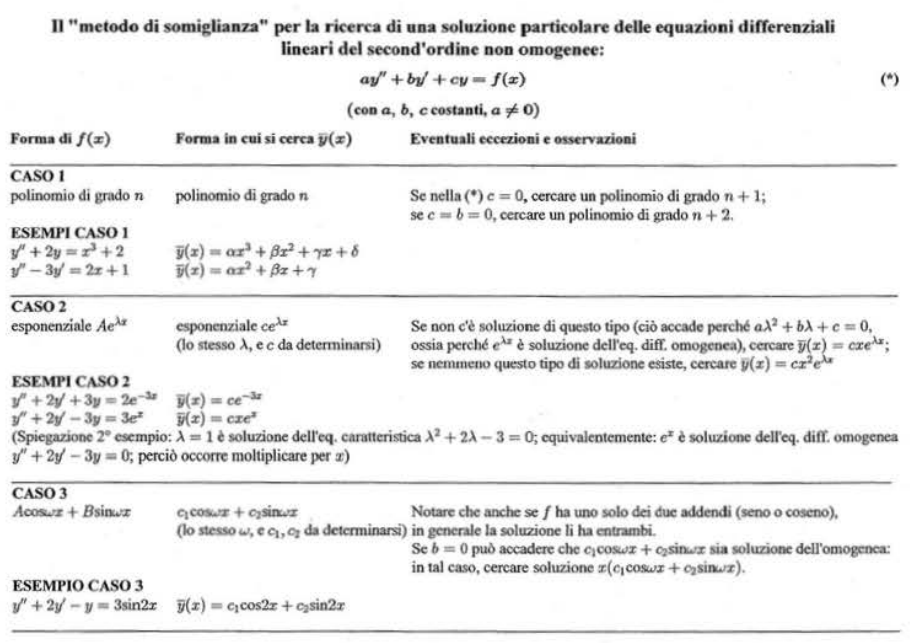
\includegraphics[height=250px]{../img/eqdiff2.PNG}
\end{center}
\begin{center}
    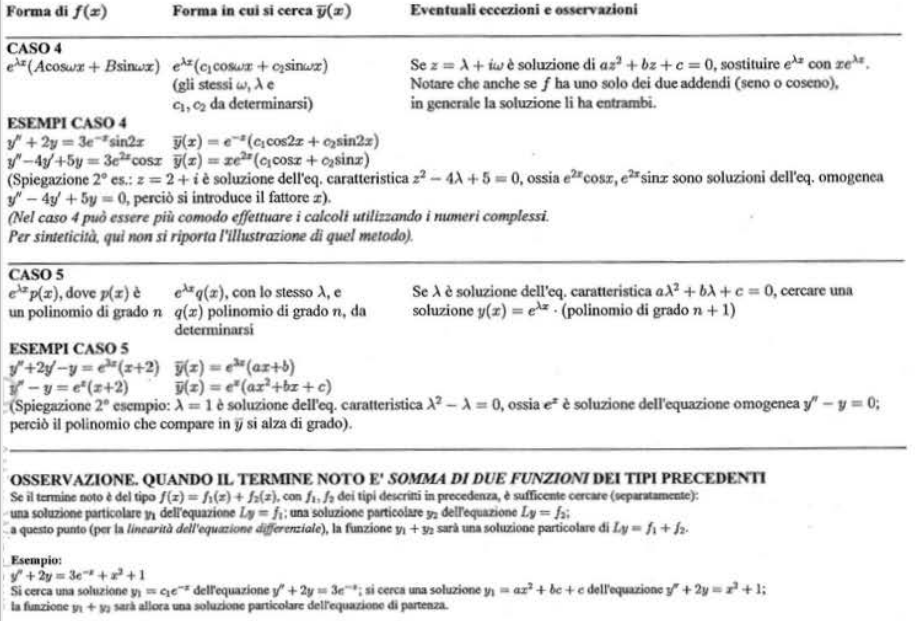
\includegraphics[height=250px]{../img/eqdiff2(1).PNG}
\end{center}